%%%%%%%%%%%%%%%%%%%%PACKAGES&STYLING&&&&&&&&&&&&&&&&&&&&&&&&&&&&&&&&&&&&&
%\documentclass{article}
\documentclass{scrartcl}
\usepackage[utf8]{inputenc}
\usepackage[english]{babel}
\usepackage{booktabs}
\usepackage{xcolor}
\usepackage{amsmath}
\usepackage{graphicx}
\usepackage{fancyhdr}
\pagestyle{fancy}
\fancyhf{}
\rhead{Assignment 5.1}
\lhead{Quadratic vs Linear least squares fit}
\rfoot{Page \thepage}
%%%%%%%%%%%%%%%%%PREAMBLE%%%%%%%%%%%%%%%%%%%%%%%%%%%%%%%%%%%%%%%%%%%%%%
\title{Machine Learning}
\subtitle{Assignment 5.1}
\author{Submitted By: Ranji Raj}
\date{\today}

\begin{document}

\maketitle
%\color{blue}
%%%%%%%%%%%%%%%%%%%%%%%%%%%%%%%%%%%%%%%%%%%%%%%%%%%%%%%%%%%%%%%%%%%%%%%%
\section*{Linear Least Squares Fit}
Given by the equation $\hat y_i=\beta_{0}+\beta_{1}x_{i}$\\

The Sum-Of-Squared-Errors is given as, $E=\sum_{i=1}^{n} (y_{i}-\hat y_{i})^{2}$\\

$E=\sum_{i=1}^{n} [y_{i}-(\beta_{0}+\beta_{1}x_{i})]^{2}$\\

Differentiating partially wrt $\beta_{1}$,\\

$$ \frac{\partial E}{\partial \beta_{1}}=2*(-x_{i})*\sum_{i=1}^{n} [y_{i}-(\beta_{0}+\beta_{1}x_{i})] $$\\

To take the minimum we equate to 0,\\

$ \sum_{i=1}^{n}(-x_{i}y_{i}+\beta_{1}x_{i}^{2}+\beta_{0}x_{i})=0$\\

Rearranging the equation we obtain,\\
\begin{equation} \label{eq:1}
\sum_{i=1}^{n}\beta_{1}x_{i}^{2}+\sum_{i=1}^{n}\beta_{0}x_{i}=\sum_{i=1}^{n}x_{i}y_{i}
\end{equation}

Similarly, differentiating partially wrt $\beta_{0}$,\\

$$ \frac{\partial E}{\partial \beta_{0}}=-2*\sum_{i=1}^{n} [y_{i}-(\beta_{0}+\beta_{1}x_{i})]$$\\

To take the minimum we equate to 0,\\

$ \sum_{i=1}^{n}(-y_{i}+\beta_{1}x_{i}+\beta_{0})=0$\\

Rearranging the equation we obtain,\\
\begin{equation} \label{eq:2}
\sum_{i=1}^{n}\beta_{1}x_{i}+\sum_{i=1}^{n}\beta_{0}=\sum_{i=1}^{n}y_{i}
\end{equation}

By standard linear algebra notation we can represent (1) and (2) in matrix form as,\\
\begin{equation}
    \begin{bmatrix} n & \sum x_{i}\\ \sum x_{i} & \sum x_{i}^{2} \end{bmatrix}
\begin{bmatrix} \beta_{0}\\ \beta_{1} \end{bmatrix} 
= \begin{bmatrix} \sum y_{i}\\ \sum x_{i}y_i \end{bmatrix}
\end{equation}

From the given data we estimate the values for (3),\\

\begin{table}[ht]
    \centering
    \begin{tabular}{|c|c|c|c|}
    \hline
        $x_i$ & $y_i$ & $x_iy_i$ & $x_i^2$ \\ [0.5ex]
    \hline \hline
        1 & 1 & 1 & 1\\
    \hline
        3 & 6 & 18 & 9\\
    \hline
        4 & 1 & 4 & 36\\
    \hline
        7 & 8 & 56 & 49\\
    \hline
        9 & 20 & 180 & 81\\
    \hline
        $\sum=24$ & $\sum=36$ & $\sum=259$ & $\sum=156$\\ [0.5ex]
    \hline
    \end{tabular}
    \caption{Data for Linear least squares fit}
    \label{tab:linear}
\end{table}

Substituting values from Table 1 in (3) we obtain, \\
$$
 \begin{bmatrix} 5 & 24\\ 24 & 156 \end{bmatrix}
\begin{bmatrix} \beta_{0}\\ \beta_{1} \end{bmatrix} 
= \begin{bmatrix} 36\\ 259 \end{bmatrix}
$$

Solving for $\beta_{0}$ and $\beta_{1}$ we obtain,
$\beta_{0}$ = -2.92 and $\beta_{1}$ = 2.11

So the equation for linear least squares fit is,\\
\begin{equation}
\hat y_i=-2.92+2.11x_i  
\end{equation}

\begin{figure}[ht]
    \centering
    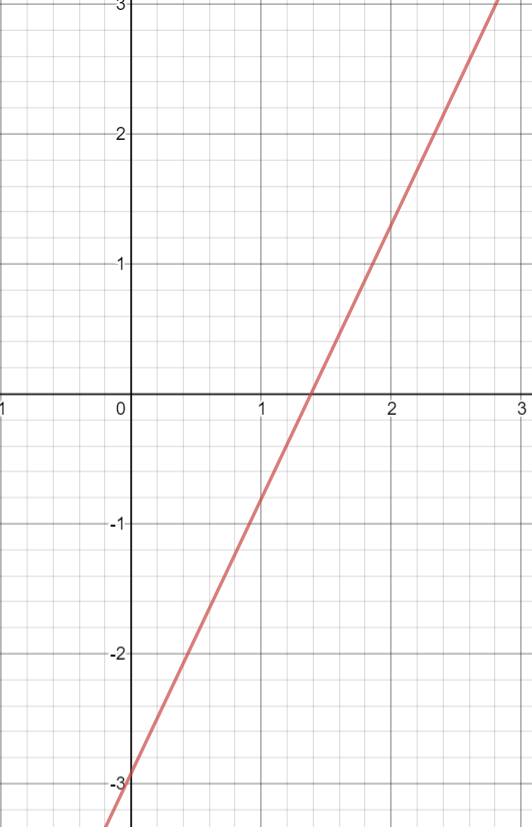
\includegraphics[width=3cm, height=3cm]{Linearfit.png}
    \caption{(a) Linear Least Squares Fit}
    \label{fig:lf}
\end{figure}

Now for each value of $x_i$ we predict $\hat y_i$ from (4)\\

We then calculate the Mean Squared Error(MSE) for our 5 data points as\\

$$MSE =\frac{\sum_{i=1}^{5}(y_i-\hat y_i)^2}{5}$$

\begin{equation}
MSE =\frac{60.667}{5}=12.13    
\end{equation}


%\fbox{\begin{minipage}{10em}
%\centering
%MSE = 12.13
%\end{minipage}}

\begin{table}[ht]
    \centering
    \begin{tabular}{|c|c|c|}
    \hline
        $x_i$ & $\hat y_i$ & $(y_i-\hat y_i)^2$ \\
    \hline \hline
        1 & -0.818 & 3.305\\
    \hline
        3 & 3.402 & 6.74\\
    \hline
        4 & 5.512 & 20.358\\
    \hline
        7 & 11.842 & 14.76\\
    \hline
        9 & 16.062 & 15.50\\
    \hline
        &  & $\sum=60.67$\\
    \hline
    \end{tabular}
    \caption{SSE for linear least squares}
    \label{tab:SSE1}
\end{table}
%%%%%%%%%%%%%%%%%%%%%%%%%%%%%%%%%%%%%%%%%%%%%%%%%%%%%%%%%%%%%%%%%%%%%%%%%%%%
\section*{Quadratic Least Squares Fit}

Given by the equation $\hat y_i=\beta_{0}+\beta_{1}x_{i}+\beta_{2}x_{i}^{2}$\\

The Sum-Of-Squared-Errors is given as, $E=\sum_{i=1}^{n} (y_{i}-\hat y_{i})^{2}$\\

$E=\sum_{i=1}^{n} [y_{i}-(\beta_{0}+\beta_{1}x_{i}+\beta_{2}x_{i}^{2})]^{2}$\\
%%%%%%%%%%%%%%%%%%%%%%%%%%%%%%%%%%%%%%%%%%%%%%%%%%%%%%%%%%%%%%%%%%%%%%%%%
Differentiating partially wrt $\beta_{0}$,\\

$$ \frac{\partial E}{\partial \beta_{0}}=-2*\sum_{i=1}^{n} [y_{i}-(\beta_{0}+\beta_{1}x_{i}+\beta_{2}x_{i}^{2})] $$\\

To take the minimum we equate to 0,\\

$ \sum_{i=1}^{n}(\beta_0+\beta_1x_{i}+\beta_{2}x_{i}^{2}-y_i)=0$\\

Rearranging the equation we obtain,\\
\begin{equation}
n\beta_{0}+\sum_{i=1}^{n}\beta_{1}x_{i}+\sum_{i=1}^{n}\beta_2x_i^2=\sum_{i=1}^{n}y_{i}
\end{equation}
%%%%%%%%%%%%%%%%%%%%%%%%%%%%%%%%%%%%%%%%%%%%%%%%%%%%%%%%%%%%%%%%%%%%%%%%%%
Similarly, differentiating partially wrt $\beta_{1}$,\\

$$ \frac{\partial E}{\partial \beta_{1}}=2*x_i\sum_{i=1}^{n} [y_{i}-(\beta_{0}+\beta_{1}x_{i}+\beta_2x_i^2)]$$\\

To take the minimum we equate to 0,\\

$ \sum_{i=1}^{n}(-x_iy_{i}+\beta_{0}x_{i}+\beta_{1}x_i^2+\beta_2x_i^3)=0$\\

Rearranging the equation we obtain,\\
\begin{equation}
\sum_{i=1}^{n}\beta_{0}x_{i}+\sum_{i=1}^{n}\beta_{1}x_i^2+\sum_{i=1}^{n}\beta_{2}x_i^3=\sum_{i=1}^{n}x_iy_{i}
\end{equation}

%%%%%%%%%%%%%%%%%%%%%%%%%%%%%%%%%%%%%%%%%%%%%%%%%%%%%%%%%%%%%%%%%%%%%%%
Similarly, differentiating partially wrt $\beta_{2}$,\\

$$ \frac{\partial E}{\partial \beta_{2}}=2*x_i^2\sum_{i=1}^{n} [y_{i}-(\beta_{0}+\beta_{1}x_{i}+\beta_2x_i^2)]$$\\

To take the minimum we equate to 0,\\

$ \sum_{i=1}^{n}(-x_{i}^2y_{i}+\beta_{0}x_{i}^2+\beta_{1}x_i^3+\beta_2x_i^4)=0$\\

Rearranging the equation we obtain,\\
\begin{equation}
\sum_{i=1}^{n}\beta_{0}x_{i}^2+\sum_{i=1}^{n}\beta_{1}x_i^3+\sum_{i=1}^{n}\beta_{2}x_i^4=\sum_{i=1}^{n}x_i^2y_{i}
\end{equation}
%%%%%%%%%%%%%%%%%%%%%%%%%%%%%%%%%%%%%%%%%%%%%%%%%%%%%%%%%%%%%%%%%%%%%%

By standard linear algebra notation we can represent (6),(7) and (8) in matrix form as,\\
\begin{equation}
    \begin{bmatrix} n & \sum x_{i} & \sum x_{i}^{2}\\
    \sum x_{i} & \sum x_{i}^{2} & \sum x_i^3\\
    \sum x_{i}^2 & \sum x_{i}^{3} & \sum x_i^4\\
    \end{bmatrix}
\begin{bmatrix} \beta_{0}\\ \beta_{1}\\ \beta_{2} \end{bmatrix} 
= \begin{bmatrix} \sum y_{i}\\ \sum x_{i}y_i \\ \sum x_{i}^2y_i \end{bmatrix}
\end{equation}

From the given data we estimate the values for (9),\\

\begin{table}[ht]
    \centering
    \begin{tabular}{|c|c|c|c|c|c|c|}
    \hline
        $x_i$ & $y_i$ & $x_iy_i$ & $x_i^2$ & $x_i^3$ & $x_i^4$ & $x_i^{2}y_i$\\ [0.5ex]
    \hline \hline
        1 & 1 & 1 & 1 & 1 & 1 & 1\\
    \hline
        3 & 6 & 18 & 9 & 27 & 81 & 54\\
    \hline
        4 & 1 & 4 & 16 & 64 & 256 & 64\\
    \hline
        7 & 8 & 56 & 49 & 353 & 2401 & 343\\
    \hline
        9 & 20 & 180 & 81 & 729 & 6561 & 729\\
    \hline
        $\sum=24$ & $\sum=36$ & $\sum=259$ & $\sum=156$ & $\sum=1164$ & $\sum=9300$ & $\sum=2083$\\
        [0.5ex]
    \hline
    \end{tabular}
    \caption{Data for Quadratic least squares fit}
    \label{tab:quad}
\end{table}

Substituting values from Table 3 in (9) we obtain, \\
$$
 \begin{bmatrix} 5 & 24 & 156\\ 24 & 156 & 1164\\ 156 & 1164 & 9300 \end{bmatrix}
\begin{bmatrix} \beta_{0}\\ \beta_{1} \\ \beta_{2} \end{bmatrix} 
= \begin{bmatrix} 36\\ 259\\ 2083 \end{bmatrix}
$$

Solving for $\beta_{0}$, $\beta_{1}$ and $\beta_{2}$ we obtain,
$\beta_{0}$ = 4.081, $\beta_{1}$ = -1.937 and $\beta_{2}$ = 0.3979

So the equation for quadratic least squares fit is,\\
\begin{equation}
\hat y_i=4.081-1.937x_i+0.3979x_i^2  
\end{equation}

\begin{figure}[ht]
    \centering
    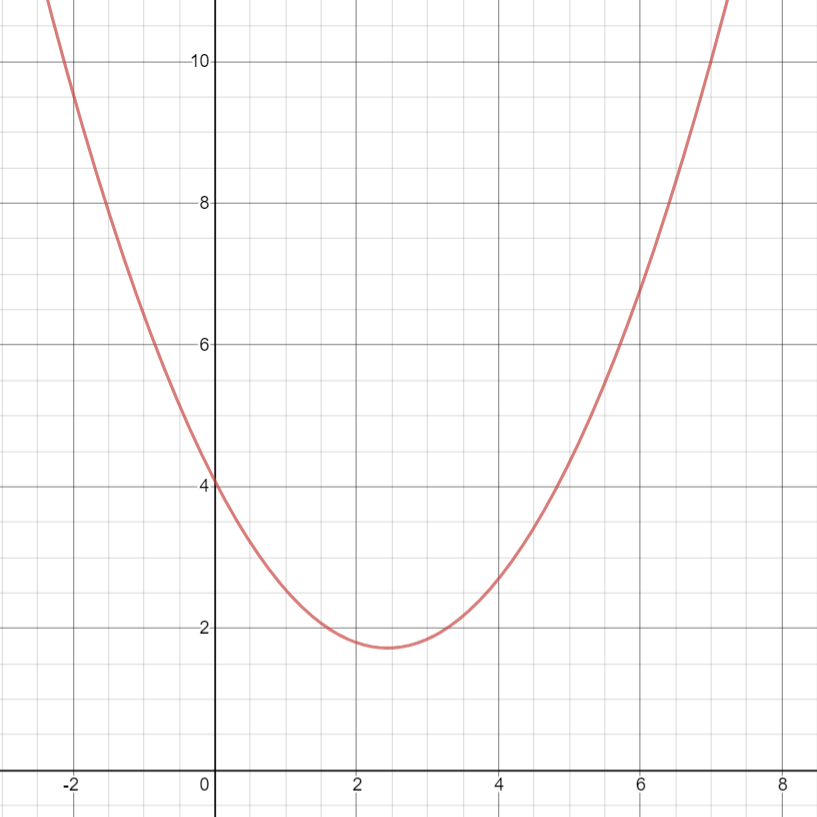
\includegraphics[width=4cm, height=4cm]{quadraticfit.png}
    \caption{(b) Quadratic Least Squares Fit}
    \label{fig:qf}
\end{figure}

Now for each value of $x_i$ and $x_i^2$ we predict $\hat y_i$ from (10)\\

We then calculate the Mean Squared Error(MSE) for our 5 data points as\\

$$MSE =\frac{\sum_{i=1}^{5}(y_i-\hat y_i)^2}{5}$$

\begin{equation}
MSE =\frac{28.2816}{5}=5.65    
\end{equation}


\begin{table}[ht]
    \centering
    \begin{tabular}{|c|c|c|}
    \hline
        $x_i$ & $\hat y_i$ & $(y_i-\hat y_i)^2$ \\
    \hline \hline
        1 & 2.54 & 2.3716\\
    \hline
        3 & 1.8 & 17.64\\
    \hline
        4 & 2.6 & 2.56\\
    \hline
        7 & 9.68 & 2.82\\
    \hline
        9 & 18.3 & 2.89\\
    \hline
        &  & $\sum=28.2816$\\
    \hline
    \end{tabular}
    \caption{SSE for quadratic least squares}
    \label{tab:SSE2}
\end{table}

Comparing (5) and (11) we observe that there is a significant \emph{plummet} in the error margin when we fit quadratic curves.\\

Conclusion:
\begin{itemize}
    \item When we fit a higher order polynomial it will try to generalize the model as much as it can so we witness a error drop when compared to linear fit.
    \item But, it is observed there is poor generalizability with the test data which leads to over-fitting with higher degree polynomials. 
\end{itemize}

\end{document}